% !TeX spellcheck = ru_ru_en_us
\documentclass[]{TAACpaper}

\begin{document}

%This is the comment. Further under the text features of use of style of theses are described

%We are specifying language of the paper
\selectlanguage{russian}
\def\dd#1#2{\frac{\partial#1}{\partial#2}}
\section{
%%%%%%%%%%%%%%% You have to specify name of your paper here
``О связи задачи маршрутизации с жесткими временными ограничениями с задачей о назначениях'' 
}

\authors{
Р.~А.~Шафеев
}

\abstract{
%%%%%%%%%%%%%%% You have to insert abstract of your paper here
В статье приводится метод определения решения задачи маршрутизации с учетом временных ограничений, которое можно использовать в вероятностном методе поиска с запретами как нижнюю границу для формирования окрестности потенциальных решений, что может значительно уменьшить время поиска оптимума. В случае если целевая функция не зависит от простоя автомобиля перед посещением следующего пункта назначения, то такое решение совпадает с оптимумом исходной задачи.
}

%%%%%%%%%%%%%%% To define new section use a command \subsection
% We are defining "Introduction" here
\subsection{Введение}
%%%%% Paragraph text. To separate paragraphs use empty lines.
Задача маршрутизации с жесткими временными ограничениями принадлежит к классу NP трудных\cite{VRPTW}, для решения которых широко применяются метаэвристические алгоритмы, в частности различные модификации алгоритма вероятностного поиска с запретами \cite{Tabu_search}. Данные алгоритмы позволяют находить качественные решения, однако при решении динамических задач маршрутизации, для которых время нахождения оптимума является критическим, малопригодны. Если  провести анализ исходных данных задачи, то часто  возникает ситуация, что граф имеет статическую структуру в не зависимости от временных ограничений и задачу можно решить за полиномиальное время \cite{Assignment_Problems}. Такое решение можно использовать, как нижнюю границу при поиске решения исходной задачи. А в случае, когда простой автомобиля перед посещением следующего клиента не влияет на целевую функцию, то такое решение совпадает с оптимумом.  

\subsection{Постановка задачи и дискретная модель}
Пусть $C,dim(C)=n$ – множество точек, соответствующих текущему положению автотранспортных средств(АТС), $Q,dim(Q)=m$ – множество пунктов назначения. $D$ $dim(D)=k$ - множество складов.\\
Пусть $V=C\cup{Q}\cup{D}$:\\
$P_i(t)={lat,lon}$, где $i\in{V}$- местоположением $i$-го узла в момент времени $t$.\\
$S_k$, где $k\in{C}$ - грузоподъемность АТС;\\
$t_{A}^{j}$ - время поступления $j$-ой заявки.\\
$\bigtriangleup\tilde{t}_{\omega}^{j}$-время обработки $j$-ой заявки на складе (прогнозируемое время обработки);\\
$\tilde{t}^{j}$-время доставки груза $j$-му клиенту (прогнозируемое время, настроечное);\\
$depot_j$-склад, на котором находится груз $j$-го клиента;\\
$\nu_j$-груз, который необходимо доставить $j$-му клиенту.

Необходимо составить оптимальные маршруты передвижения АТС для посещения всех пунктов назначения.

Зададим последовательность неизвестных матриц $\{X^k\}^n_{k=1}$, элементы  которых принимают следующие значения:
\begin{equation}
  x^{(k)}_{i,j} = 
    \begin{cases}
	  1,&\text{авт. $k$ движется из $i$-го узла в $j$-й, 
	           $i\in{C}\cup{Q}\cup{D}, j \in Q\cup{D}$ }\\
	  0,&\text{в противном случае.}
    \end{cases}
\end{equation}
Целевая функция примет следующий вид:
\begin{equation} \label{main_objective}
  F(X) = 
    \sum_{k \in C}
     \sum_{i,j\cup{V}} 
     x_{ij}^{k}\cdot\Omega_{ij}+\sum_{j\in{Q}}\tau(j)
     \to min
\end{equation}
При ограничениях:
\begin{align} 
& \sum_{i\in{V}}x_{ij}^{k}=y_{j,d}^{k}, \forall{k}\in{C}, \forall{j}\in{Q},\forall{d}\in{D}\\
& sign[\sum_{j\in{Q}}y_{j,d}^{k}]=\sum_{i\in{V}}x_{i,d}^{k}, \forall{k}\in{C}, \forall{d}\in{D}
& \sum_{k \in C}\sum_{j \in Q}x^{(k)}_{i,j} = 1, 
  \forall i \in C \cup Q, \forall k \in C \label{main_cond_1}\\ 
& \sum_{j \in Q} ( 
       x^{(k)}_{k,j} -x^{(k)}_{i,j} ) \geq 0, 
       \forall i \in Q ,  \forall k \in C \label{main_cond_2}\\
& \sum_{i \in Q \cup  \{k\}} x^{(k)}_{i,\omega} - 
  \sum_{j \in Q} x^{(k)}_{\omega,j} = 0, 
  \forall \omega \in Q ,  \forall k \in C \label{main_cond_3}\\
&  \sum_{i \in S}\sum_{j \notin S}x^{(k)}_{i,j} > 0, 
  S=\{s \in Q: \sum_{j \in Q \cup C}x^{(k)}_{j,s}>0 \}  ,\forall k \in C \label{main_cond_4}\\
& t_j \leq \tilde{t_j} \leq t_j + \Delta t_j, \forall j \in Q, 
\tilde{t_j} \text {- время прибытия в j-й пункт назначения} \label{main_cond_5}
\end{align}

\subsection{Анализ исходных данных}
В случае, когда простой автомобиля перед посещением следующего клиента не влияет на целевую функцию, а именно $\varphi=const=0$, тогда в некоторых случаях временные ограничения могут не влиять на структуру графа и задача сводится к задаче о назначениях. В силу того, что $NP \neq P$, однозначный переход невозможен, но из-за наличия временных ограничений граф задачи может не иметь локальных циклов и в этом случае  ограничения (\ref{main_cond_4}) и (\ref{main_cond_5}) возможно опустить после удаления дуг $(i,j)$ по которым невозможно достижение вершины $j$ в не зависимости от времени прибытия в вершину $i$.

Для того, чтобы проверить возможность такого перехода, введем дополнительные величины. 
\begin{enumerate}
\item Учитывая наложенные на целевую функцию ограничения, время прибытия в $j$–й пункт назначения равно:
\begin{equation} \label{t_j_input}
   \exists h_i \in [0,1] : \tilde{t_i} = t_i + h_i \cdot \Delta t_i
\end{equation}

\item Введем матрицу $U$, элементы которой показывают в количественной форме нарушение временного окна:
\begin{equation} \label{matrix_U}
 U(\vec{h}) : u_{i,j} = 
    \begin{cases}
	  0, i=j, \\
      t_i + h_i \cdot \Delta t_i + \omega_i + t_{i,j} - t_j - \Delta t_j, i \neq j
    \end{cases}   
\end{equation}
\end{enumerate}

Можно сказать, что если элемент матрицы $U(\vec{h}=\vec{1})$ отрицательный, то передвижение между пунктами возможно выполнить в не зависимости от временных ограничений. Поэтому построим граф $G$ для задачи маршрутизации, в котором уже будут учтены ограничения (\ref{main_cond_4}) и (\ref{main_cond_5}), задав следующую матрицу инцидентности:
\begin{equation} \label{matrix_I}
 I(\vec{h}) : I_{i,j} = 
    \begin{cases}
	  0, &\text{если $u_{i,j} \geq 0$,} \\
      1, &\text{если $u_{i,j}<0$}
    \end{cases}, i \in C \cup Q, j \in Q
\end{equation}
\newtheorem{Def}{Определение} 
\begin{Def}\label{def_main}
Если:
  \begin{enumerate}
  \item $\varphi=const=0$;
  \item матрица $I(\vec{0})$ равна матрице $I(\vec{1})$;
  \item граф $G$, построенный по матрице инцидентности $I(\vec{0})$ не является мультиграфом,
  \end{enumerate}
 тогда задача маршрутизации с жесткими ограничениями по времени сводится к задаче о назначениях.
\end{Def}
Это утверждение вытекает из следующих лемм.

\newtheorem{Lem}{Лемма}
\begin{Lem}
Если матрица $I(\vec{0}) = I(\vec{1})$, тогда $I(\vec{0})=I(\vec{h}), \forall \vec{h}: h_i \in [0,1]$
\end{Lem}
Доказательство. 
Элементы матрицы $I_{i,j}$ не зависят от вектора $\vec{h}$ при $i \in C, j \in Q$, так как вершины из множества C соответствуют местоположениям автомобилей в начальный момент времени и им не заданы временные окна ($\Delta t_i = 0, \forall i \in C$). Остальные элементы матрицы можно представить в виде формулы:
\begin{equation} 
I_{i,j}(h_i) = \frac{1 - sign(u_{i,j}(h_i))}{2}
\end{equation}
По условию $I(\vec{0}) = I(\vec{1})$, тогда:

\begin{flalign*}
&\frac{1 - sign(u_{i,j}(0))}{2} =  \frac{1 - sign(u_{i,j}(1))}{2} \Rightarrow
sign(u_{i,j}(0)) = sign(u_{i,j}(1))&
\end{flalign*}
Или:
\begin{flalign*}
&\left[\begin{array}{l}
     \begin{cases}
	  u_{i,j}(0)>0  \\
      u_{i,j}(1)>0
    \end{cases}\\
    \begin{cases}
	  u_{i,j}(0)<0  \\
      u_{i,j}(1)<0
    \end{cases}
\end{array}\right.&
\end{flalign*}

Функция $u_{i,j}(h_i)$ на промежутке $h_i \in [0,1]$ является монотонно возрастающей, потому что производная $\dd{u_{i,j}(h_i)}{h_i} = \Delta t_i >0$ положительна на всем промежутке. Поэтому:

\begin{flalign*}
&\left[\begin{array}{l}
     \begin{cases}
	  u_{i,j}(0)>0  \\
      u_{i,j}(1)>0
    \end{cases} \Rightarrow u_{i,j}(h_i)>0 \\
    \begin{cases}
	  u_{i,j}(0)<0  \\
      u_{i,j}(1)<0
    \end{cases} \Rightarrow u_{i,j}(h_i)<0
\end{array}\right.
\Rightarrow sign(u_{i,j}(0)) = sign(u_{i,j}(h_i)), \forall h_i \in [0,1] &
\end{flalign*}
Тогда $sign(u_{i,j}(0)) = sign(u_{i,j}(h_i)) \Rightarrow  I(\vec{h})=I(\vec{0})$. Доказано.

\newtheorem{Lem2}{Лемма}
\begin{Lem}
Если граф  $G$, построенный по матрице инцидентности $I(\vec{h}=const)$ не является мульграфом, то такой граф не имеет циклов.
\end{Lem}
Доказательство(от противного). Пусть дан граф $G(V={C \cup Q}, E)$, построенный по матрице инцидентности  $I(\vec{h}=const)$ и в нем имеется цикл: \begin{align*}
&E_{cicle}=\{(v_{s_1},v_{s_2}),(v_{s_2},v_{s_3}),...,(v_{s_{k-1}},v_{s_k}),(v_{s_k},v_{s_1})\}
\end{align*}
Предположим, что при наличии цикла $E_{cicle}$ в графе $G$ нет дуги $(v_{s_1},v_{s_k})$, т.е. АТС не успеет добраться из вершины $v_{s_1}$ в вершину $v_{s_k}$ не нарушив временные ограничения. Поэтому:
\begin{equation} \label{error_inequality}
 t_{s_k} + \Delta t_{s_k} <  \tilde{t}_{s_1} + \omega_{s_1} + t_{s_1,s_k}
\end{equation}
Согласно предположению о существовании цикла $E_{cicle}$ верно следующее неравенство ( $E_{route}=E_{cicle} / \{(v_{s_k},v_{s_1}) \}$):
\begin{equation} \label{time_s_k_inequality}
 t_{s_k} + \Delta t_{s_k} > \tilde{t}_{s_{k-1}} + \omega_{s_{k-1}} + t_{s_{k-1},s_k} = \tilde{t}_{s_1} +  \sum_{(i,j) \in E_{route}} (t_{i,j} +  \omega_{s_i}) = A
\end{equation}
Пусть передвижение от вершины $v_{s_1}$ в вершину $v_{s_k}$ будет выполняться по дугам $E_{route}$. Тогда:
\begin{equation} \label{time_route}
 \tilde{t}_{s_1} + \omega_{s_1} + t_{s_1,s_k} \leq \tilde{t}_{s_1} + \omega_{s_1} + \sum_{(i,j) \in E_{route}} t_{i,j} \leq A
\end{equation}
Подставим (\ref{time_route}) в (\ref{time_s_k_inequality}):
\begin{equation} \label{true_inequality}
 t_{s_k} + \Delta t_{s_k} > \tilde{t}_{s_1} + \omega_{s_1} + t_{s_1,s_k}
\end{equation}
Пришли к противоречию, следовательно, неравенство (\ref{error_inequality}) неверно. Доказано.

\subsection{Переход к задаче о назначениях}
Если выполняются правила из определения \ref{def_main}, тогда можно свести исходную задачу к задаче о назначениях.

Введем замену переменных X :
\begin{equation} \label{y_replace}
\forall k \in C: ~Y^k = \{ I_{i,j}(0) \cdot x^{(k)}_{i,j} , i \in Q \cup  \{k\} , j \in Q  \}
\end{equation}

Теперь задачу можно сформулировать таким образом, что ее можно разрешить за полиномиальное время:
\begin{align} 
  &F(Y) = 
    \sum_{k \in C}
     \sum_{i \in Q \cup  \{k\},j \in Q} 
     \Omega_{i,j}\cdot y^{(k)}_{i,j})
     \to min\\
& \sum_{k \in C}\sum_{j \in Q}y^{(k)}_{i,j} = 1, 
  \forall i \in C \cup Q, \forall k \in C \label{mod_cond_1}\\ 
& \sum_{j \in Q} ( 
       y^{(k)}_{k,j} -y^{(k)}_{i,j} ) \geq 0, 
       \forall i \in Q ,  \forall k \in C \label{mod_cond_2}\\
& \sum_{j \in Q \cup  \{k\}} y^{(k)}_{i,\omega} - 
  \sum_{i \in Q} y^{(k)}_{\omega,j} = 0, 
  \forall \omega \in Q ,  \forall k \in C \label{mod_cond_3}
\end{align}

Чтобы получить задачу о назначениях в классическом ее виде, построим на основе графа $G$ двудольный граф $G_b(V_{begin},V_{end},E_b)$ по следующему принципу:
\begin{enumerate}
\item $V_{begin} = \{v \in C \cup Q\ : \exists (v,\omega) \in E, \omega \in Q \}$ - состоит из множества вершин, для которых найдется хотя бы одна выходящая дуга из множества E;
\item $V_{end} = \{v  \in Q\ : \exists (\omega,v) \in E, \omega \in C \cup Q \}$ - состоит из множества вершин, для которых найдется хотя бы одна входящая дуга из множества E;
\item $E_b = \{(v,\omega) \in E: v \in V_{begin}, \omega \in V_{end} \}$.
\end{enumerate}

\begin{figure}[h]
\hfil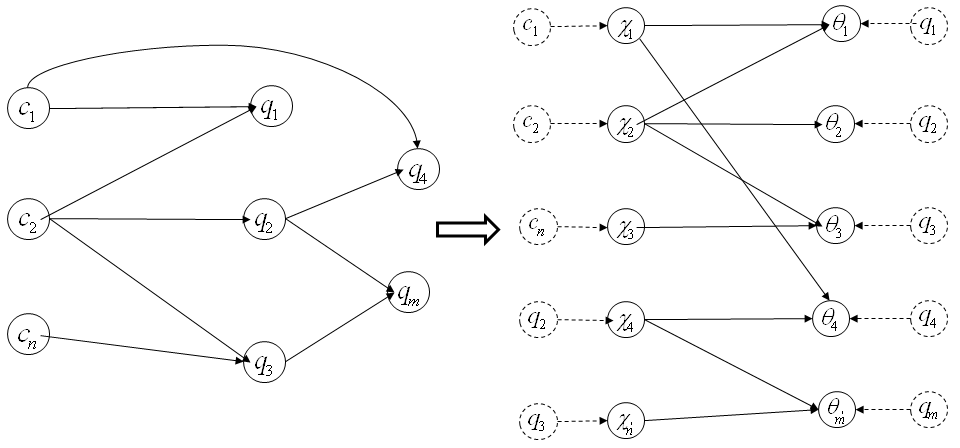
\includegraphics[height=2.0in]{sign_graph}\hfil
\caption
{
  Пример преобразования графа $G$ в двудольный граф $G_b$.
}
\label{aba:fig1}
\end{figure}

\subsection{Результаты}
Преобразованную задачу(рис. \ref{aba:fig1}) рекомендуется решать с помощью метода Голдберга и Кеннеди,  основанного на технике масштабирования при переходе к задаче поиска потока минимальной стоимости \cite{Goldberg_Kennedy}. Сложность алгоритма равна $O(\sqrt{n}mlog(nC))$.

В случае, если функция $\varphi(t)$ присутствует в целевой функции, то решение преобразованной задачи может послужить нижней границей, которую можно использовать для отсеивания заведомо худших решений при формировании окрестности вокруг текущего решения в работе вероятностного алгоритма поиска с запретами.

Проверка метода была выполнена на тестовых задачах Кристофидеса, Голдберга  и Тейларда с временными ограничениями, удовлетворяющими условиям, которые были изложены в определении \ref{def_main} \cite{problems_Christofides,problems_Golden,problems_Taillard}.    

\subsection{Выводы}
Предложены правила перехода от задачи маршрутизации с учетом временных ограничений к задаче о назначениях. Данную технику целесообразно использовать для задач маршрутизации, в которых не учитывается простой автомобиля. Также  метод можно использовать для инициализации метаэвристического алгоритма или в виде более качественной нижней границы для определения оптимума. 


\begin{thebibliography}{99}
%In brackets we writes the name which is used for referencing.

\bibitem{VRPTW} T.~Babb, Pickup and Delivery Problem with Time Windows // Coordinated Transportation Systems: The State of the Art. Department of Computer Science University of Central Florida Orlando, Florida, 2005, 38 p.

\bibitem{Tabu_search} O.~Braysy, M.~Gendreau, Vehicle Routing Problem with Time Windows, Part I: Route Constuction and local algorithms // Transportation science Vol.39 No. 1, 2005, p. 104-118.

\bibitem{Assignment_Problems} E.~Rainer, Assignment problems, 2009, 402 p. 

\bibitem{Goldberg_Kennedy} V.~Goldberg, R.~Kennedy, An Efficient cost scaling algotirhm for the assignment problem, Math. Program., 1995, p. 153--177.  

\bibitem{problems_Christofides}  N. Christofides, S. Eilon, An algorithm for the vehicle dispatching problem //Operational Research Quarterly, 20, 1969, p. 309–318.
\bibitem{problems_Golden}  B. Golden, E. Wasil, J. Kelly, I-M. Chao. The impact of metaheuristics on solving the vehicle routing problem: Algorithms, problem sets, and computational results. In T. Crainic and G. Laporte, editors // Fleet Management and Logistics, Kluwer, Boston, 1998 p. 33–56.
\bibitem{problems_Taillard}  E. Taillard. VRP benchmarks.\\ http://mistic.heig-vd.ch/taillard/problemes.dir/vrp.dir/vrp.html, 1993.
\end{thebibliography}

\subsection{Автор}
\author{Роман Александрович Шафеев}{магистр 2-го года обучения, факультет информатики и управления, Национальный технический университет <<Харьковский политехнический институт>>, Харьков, Украина}
{rs@premiumgis.com}


\end{document} 